
\section{Synthèse de mouvements par optimisation\label{sec:motion_generation}}

\subsection{Motivations}

Dans le contexte de la compétition RoboCup, différentes catégories de
mouvements sont à l'oeuvre. Les mouvements de relevage depuis
la posture couchée face avant et face arrière.
Ces mouvements sont lents et quasiment statiques.
À l'inverse, les mouvements de marche omnidirectionnelle et 
de tir dans la balle sont des mouvements très dynamiques,
où la stabilité bipède est une contrainte majeure.

Actuellement, les mouvements de relevage et de tir 
sont entièrement en boucle ouverte. 
Avant même leur exécution, les trajectoires de 
toutes les articulations du robot sont complètement déterminées.
Le mouvement de marche (\textit{IKWalk} ou \textit{QuinticWalk}),
même stabilisé grâce aux capteurs de pression, se base
également sur des trajectoires de références en boucle ouverte.
À noter que jusqu'en 2016, le mouvement de tir était en boucle fermée et 
se stabilisait à l'aide des capteurs de pression, de l'IMU et d'un 
modèle géométrique du robot.
Bien que très puissant, ce mouvement était également particulièrement 
couteux en terme d'efforts humains à régler sur chacun des robots.

Quelle soit en boucle ouverte ou en boucle fermée, la forme de 
tous les mouvements créés sur le robot Sigmaban a toujours 
été élaborée manuellement par \og expertise \fg humaine.
La stabilité et les performances des mouvements sont assurées
par le réglage à la main des nombreux paramètres laissés libres
par expérimentation (essai-erreur) sur le robot réel ; 
et ce à intervalles réguliers.
L'évolution constante des déformations mécaniques des robots ainsi que
leurs différentes imperfections expliquent le succès pratique 
de cette approche.

Cependant, au vu du temps humain consacré à ce processus, 
il est intéressant de tenter d'expérimenter une méthode de 
génération des mouvements plus \og automatique \fg.
Il s'avère en pratique qu'une fois réglés correctement, 
les mouvements en boucle ouverte atteignent des performances satisfaisantes
au regard de leur application dans le contexte RoboCup.
C'est pourquoi dans ces travaux, il a été choisi de générer 
des mouvements également en pure boucle ouverte.\\

Dans un premier temps, cette synthèse de mouvement se concentre 
sur le problème plus simple du tir. Ce problème est intéressant car : 
\begin{itemize}
    \item Il s'agit, contrairement à la marche d'un mouvement \textit{épisodique}
        n'accumulant pas les erreurs de suivi de trajectoire à chaque cycle.
        De plus, il n'y a en théorie qu'un seul choc avec le sol à considérer.
    \item Ce mouvement pour être puissant\footnote{La puissance du tir fait ici référence
        à la distance maximale parcourue par la balle. 
        Cette distance est fortement dépendante de la surface au sol. 
        Par exemple sur l'herbe artificielle, même le sens des brins d'herbe 
        affecte significativement la longueur du tir.} 
        doit nécessairement être dynamique.
        Comme pour la marche, un compromis doit être trouvé entre 
        la contrainte forte de la stabilité bipède et la performance du mouvement.
    \item Dans le contexte de la compétition RoboCup, il y a également le besoin
        d'avoir un mouvement de tir plus paramétrable ; avec une gamme variable
        de puissances, de positionnements de la balle, voir de directions de tir.
        Ceci afin d'augmenter les possibilités stratégiques de jeu.
        Or, le réglage et la maintenance manuel d'un ensemble important 
        de mouvements de tir différents est trop couteux en temps.
\end{itemize}
L'équipe Rhoban considère deux mouvements de tir distincts : le tir
classique \og droit \fg vers l'avant et le tir \og latéral \fg
envoyant la balle perpendiculairement au robot.
Seul le tir droit est ici traité.
Les mouvements de tir peuvent aussi être regroupés en deux grandes
catégories :
\begin{itemize}
    \item Les tirs en \textit{double support}.
        Initialement, le robot est immobile sur ses deux pieds, 
        les genoux pliés en posture de marche.
        Le robot soulève le pied de tir et passe en simple support.
        Il propulse la balle et repose le pied au sol pour terminer 
        en double support les deux pieds au sol.
        Il y a donc une collision du pied avec le sol.
    \item Les tirs en \textit{simple support}.
        Initialement, le robot est immobile en équilibre statique sur un pied.
        Le pied en l'air propulse la balle puis se replace toujours 
        en restant en l'air. Durant l'intégralité du mouvement, 
        le robot reste en phase de simple support. 
        Il n'y a pas de collision avec le sol.
\end{itemize}
Pour que le tir en simple support soit réalisable, 
il faut également pouvoir générer un mouvement de passage de
double en simple support et inversement.
Initialement le robot est immobile sur ces deux pieds, 
les genoux pliés en posture de marche.
Le mouvement de passage en simple support amène le robot dans une posture
statiquement stable sur un seul pied.

Le tir en simple support stable est dans la pratique le plus simple 
à synthétiser. Ni le double support, ni la collision avec le sol
ne sont à considérer.
Le mouvement de passage en simple support nécessite la gestion 
de la dynamique en phase de double support. 
Ce mouvement est également simple à générer car il n'y a pas de collision avec 
le sol. Il n'est pas non plus très dynamique.
Le mouvement de tir en double support est le plus difficile à concevoir.
Dans ces travaux, la synthèse de ces trois mouvements est étudiée.

\subsection{Mouvement de tir expert}

Depuis 2016, le mouvement de tir utilisé par l'équipe Rhoban lors
de la compétition RoboCup est un tir en boucle ouverte et en double support.
Exprimé de manière hybride, à la fois dans l'espace articulaire
et dans l'espace cartésien, il défini des trajectoires articulaires 
affines par morceaux, parfois discontinues.
La forme du mouvement ainsi que ces paramètres sont manuellement 
ajustés par expérimentation sur le robot réel.

Après cette longue phase \og d'optimisation \fg manuelle, 
il s'avère que ce tir est particulièrement puissant tout en restant stable. 
Il parvient a exploiter au maximum les capacités des servomoteurs.
En effet, il tend à saturer le contrôle proportionnel des moteurs 
qui fonctionnent alors à leur couple maximum. 
Ce comportement limite est d'ailleurs difficile à modéliser car il met en 
évidence de nombreuses imperfections électriques.
Enfin, l'expérience a montré que ce tir fonctionnait sur plusieurs robots 
Sigmaban et était dans une certaine limite robuste aux modifications mécaniques.

Sans jamais être égalé, ce mouvement sert donc de référence et de point de
comparaison tout au long de ces travaux.
        
\subsection{Représentation des mouvements\label{sec:motion_representation}}

\begin{table}[htb]
\begin{center}
    \begin{tabular}{|p{6cm}|p{8cm}|}
        \hline
        Description de la trajectoire & Nommage\\
        \hline
        Pied de support courant. 
        ($1$ si pied gauche, $0$ si pied droit) &
        \textit{is\_left\_support\_foot} \\
        \hline
        État de support,
        utilisé pour le calcul de la dynamique inverse.
        ($0$ pour simple support, $1$ pour double support) &
        \textit{is\_double\_support} \\
        \hline
        Position cartésienne du buste 
        dans le repère du pied de support &
        \textit{trunk\_pos\_x} \newline
        \textit{trunk\_pos\_y} \newline
        \textit{trunk\_pos\_z} \\
        \hline
        Orientation du buste dans le repère
        du pied de support &
        \textit{trunk\_axis\_x} \newline
        \textit{trunk\_axis\_y} \newline
        \textit{trunk\_axis\_z} \\
        \hline
        Position cartésienne de l'autre pied 
        dans le repère du pied de support &
        \textit{foot\_pos\_x} \newline
        \textit{foot\_pos\_y} \newline
        \textit{foot\_pos\_z} \\
        \hline
        Orientation de l'autre pied dans le repère
        du pied de support &
        \textit{foot\_axis\_x} \newline
        \textit{foot\_axis\_y} \newline
        \textit{foot\_axis\_z} \\
        \hline
    \end{tabular}
    \caption{\label{tab:cart_dofs}
        Description des $12+2$ trajectoires
        définissant un mouvement dans l'espace cartésien.
        Chacune des trajectoires est représentée par une
        spline polynomiale quintique de la durée du mouvement.
    }
\end{center}
\end{table}

Dans cette étude, il a été choisi de représenter
les trajectoires des mouvements désirés sous la forme de 
splines polynomiales de degré $5$ (quintiques).
Ces trajectoires sont de plus décrites dans l'espace cartésien.
Cette représentation a plusieurs avantages :
\begin{itemize}
    \item Le calcul à tout instant des positions, 
        vitesses et accélérations désirées est simple et rapide.
    \item Les splines quintiques permettent un recollement
        à l'ordre $3$ des polynômes. Les accélérations
        et donc les couples issus de la dynamique inverse 
        sont ainsi continus.
    \item Les trajectoires sont paramétrées avec les temps,
        positions, vitesses et accélérations
        définissant chaque point de contrôle de la spline.
        L'intérêt majeur de tous ces paramètres est qu'ils sont 
        interprétables avec une vrai signification cinématique.
        Ceci simplifie grandement l'écriture de gabarits 
        (\textit{templates}) ayant pour objectif de contraindre
        la forme du mouvement pour réduire l'espace de recherche.\\
\end{itemize}

Un mouvement est donc constitué d'un ensemble de trajectoires
définissant en fonction du temps le comportement désiré du robot
dans l'espace cartésien.
La liste et le nommage dans l'implémentation des $12+2$ trajectoires
sont donnés par le tableau \ref{tab:cart_dofs}.
Pour simplifier l'espace de recherche, seul le mouvement 
des jambes est considéré. Les bras et la tête du robot ne sont
pas contrôlés et restent fixes dans la position \og zéro \fg.
Les jambes définissent un total de $12$ degrés de liberté articulaires,
que l'on retrouve avec $12$ trajectoires dans l'espace cartésien.

Les deux positions ($2\times3$ valeurs) et les deux orientations ($2\times3$ valeurs) 
du buste et du pied en vol du robot sont exprimées dans le repère du pied de support.
Son intérêt est que ce repère est fixe sur le sol et dans le monde.
Par contre, à chaque changement de pied de support,
les $12$ trajectoires cartésiennes sont alors nécessairement 
discontinues car devant être exprimées dans le repère de l'autre pied.
Le pied en vol et le pied de support sont inversés.
Les deux trajectoires supplémentaires imposent le pied de support utilisé 
ainsi que l'état en simple ou double support.
Cette information est utilisée pour choisir quel calcul de la dynamique inverse
faire intervenir (voir sections \ref{sec:dynamics_models} et \ref{sec:dynamics_constraints}).

Les positions sont représentées par les trois composantes $(x,y,z)$ de la translation
amenant le centre du pied de support au centre du repère lié au buste ou au pied en vol.
Les orientations sont quant à elles représentées par les trois composantes
d'un vecteur de rotation. Cette représentation des rotations de l'espace est 
détaillée en annexe à la section \ref{sec:axis_angle}.
Rapidement, les rotations de l'espace sont définies par un axe de rotation et un angle,
encodés dans la direction et la norme du vecteur de rotation.
Cette représentation réduit l'orientation à seulement $3$ coefficients et évite les 
configurations singulières des angles de Cardan.\\

Chacune des trajectoires formant les mouvements (tableau \ref{tab:cart_dofs})
est représentée à l'aide d'une spline polynomiale quintique.
Plus en détail, il s'agit d'une fonction du temps, polynomiale par morceaux.
Chaque morceau étant un polynôme $\mathcal{P}$ de degré $5$ défini
sur un intervalle de temps donné et caractérisé par ses $6$ 
coefficients $a_0,...,a_5 \in \mathbb{R}$ : 
$$
\mathcal{P} : t \longmapsto \sum_{i=0}^{5} a_it^i
$$
Avec $6$ \og degrés de liberté \fg, un polynôme quintique
est complètement défini par la donnée de sa valeur, sa dérivée première 
et de sa dérivée seconde ; correspondant respectivement à la position, 
la vitesse et l'accélération de la trajectoire\footnote{Par abus de langage, 
nous parlerons de position, vitesse et accélération du polynôme.}
en deux points du temps.

La spline est ainsi définie par un ensemble de points de contrôle 
trié par temps croissant :
$$
\left(
t_i, p_i, \dot{p}_i, \ddot{p}_i
\right)
\in \mathbb{R}^4
$$
avec $p_i, \dot{p}_i, \ddot{p}_i$ respectivement la position, la vitesse
et l'accélération (dérivées première et seconde) de la fonction au temps $t_i$.

L'interpolation des polynômes est calculée de la manière suivante.
Pour simplifier les calculs, chaque polynôme est en réalité défini
sur l'intervalle $[0,t]$.
Ses extrémités sont imposées par :
$$
(0,p_0,\dot{p}_0, \ddot{p}_0),(t, p_t,\dot{p}_t, \ddot{p}_t)
$$
Les coefficients du polynôme sont alors déterminés par les expressions :
\begin{gather*}
a_0 = p_{0} \\
a_1 = \dot{p}_{0} \\
a_2 = \frac{\ddot{p}_{0}}{2} \\
a_3 = -\frac{-\ddot{p}_{t}t^2+3\ddot{p}_{0}t^2+8\dot{p}_{t}t+12\dot{p}_{0}t-20p_{t}+20p_{0}}{2t^3} \\
a_4 = \frac{-2\ddot{p}_{t}t^2+3\ddot{p}_{0}t^2+14\dot{p}_{t}t+16\dot{p}_{0}t-30p_{t}+30p_{0}}{2t^4} \\
a_5 = -\frac{-\ddot{p}_{t}t^2+\ddot{p}_{0}t^2+6\dot{p}_{t}t+6\dot{p}_{0}t-12p_{t}+12p_{0}}{2t^5} \\
\end{gather*}
Au moment de l'évaluation de la spline, le morceau 
associé au temps en entrée est recherché par dichotomie 
puis le polynôme correspondant est évalué.\\

\begin{figure}[htb]
    \begin{center}
        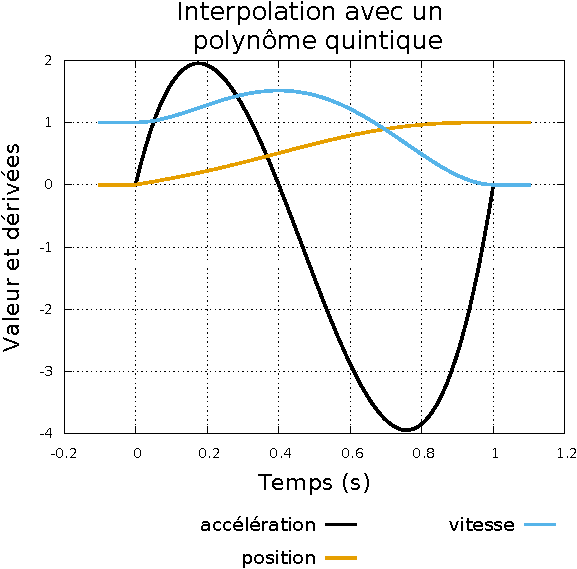
\includegraphics[type=pdf,ext=.pdf,read=.pdf,width=0.6\linewidth]{../plot/quintic_runge}
        \caption{\label{fig:quintic_runge}
            Position, vitesse et accélération d'un polynôme de degré $5$ 
            interpolé entre deux points
            de contrôle : $(t_0=0,p_0=0,\dot{p}_0=1,\ddot{p}_0=0)$ et 
            $(t=0,p_t=1,\dot{p}_t=0,\ddot{p}_t=0)$.
            La vitesse n'est pas strictement décroissante.
        }
    \end{center}
\end{figure}

Le principal inconvénient inhérent aux polynômes
vient de la manifestation du phénomène de Runge.
En imposant position, vitesse et accélération aux deux
extrémités d'un morceau de polynôme, les courbes obtenues
ne sont pas celles que l'on désireraient pour représenter les mouvements.
Un exemple typique est donné sur la figure \ref{fig:quintic_runge}.
Un mouvement initialement à vitesse constante (accélération nulle)
est amené à l'arrêt (vitesse et accélération nulle) en un
temps et à une position fixés.
On remarque que la courbe de vitesse (bleue) obtenue n'est malheureusement 
pas strictement décroissante. 
Idéalement, un mouvement de mise à l'arrêt décélérerait sans avoir besoin
d'augmenter sa vitesse. 
Ceci est cependant impossible avec des polynômes quintiques.\\

L'utilisation de primitives de mouvements dynamiques 
(\textit{Dynamic Movement Primitives}, DMP) a également été expérimentée.
Proposées par \cite{schaal_learning_2005}, le mouvement est représenté
par un système dynamique dont la position cible est vu comme 
un attracteur du système.
Des noyaux (kernels) gaussiens sont utilisés au niveau de 
l'accélération pour influencer la forme de la trajectoire.
Cette représentation possède de nombreuses propriétés intéressantes
(attraction de la trajectoire de référence (boucle fermée), 
indépendance aux décalages de position, synchronisation des degrés de liberté).
Elle est surtout employée dans le contexte de l'apprentissage par démonstration.

L'implémentation de splines de DMP a été effectuée\footnote{Voir le code source : 
\url{https://github.com/RhobanProject/Model/tree/master/DMP}} en gardant le même
formalisme (présenté ci-dessus) des points de passage.
Cette implémentation se base en partie sur l'extension de la formulation
des DMP proposée par \cite{kober_movement_2010}
permettant d'imposer position, vitesse et accélération aux extrémités
de chaque DMP.

Cette représentation n'a toutefois pas été retenue.
Le grand nombre de ses paramètres ralentit considérablement le
processus d'optimisation sans gradient (boite noire)\footnote{Les DMP sont avant tout 
spécifiquement conçus pour permettre un apprentissage du mouvement 
se basant sur le gradient.}.
De plus une grande partie de ses paramètres (les poids associés aux noyaux gaussiens) 
n'ont pas de signification géométrique.
Il est alors très difficile de contraindre efficacement la forme du mouvement 
afin de réduire l'espace de recherche.

Toujours en gardant le même formalisme (en imposant des positions, 
vitesses et accélérations), une très bonne représentation de la trajectoire 
est proposée par \cite{broquere2008soft}, \cite{broquere2011planification}.
La trajectoire \og optimale \fg est exprimée en \textit{bang-bang} sur le jerk 
et forme donc des accélérations en trapèze.
Tout l'intérêt et la difficulté de leur travaux résident dans le calcul (rapide) 
de la trajectoire (en sept étapes au niveau du jerk) permettant d'imposer 
position, vitesse et accélération aux deux extrémités de la trajectoire.
Ceci tout en assurant des bornes sur la valeur absolue 
des vitesses, accélérations et jerks.
À noter que ces travaux ont été étendus par \cite{zhao2015trajectory} afin
de correctement synchroniser plusieurs degrés de liberté ensemble.
À l'implémentation près, ces travaux sont directement applicables ici
en remplacement des polynômes quintiques.

\subsection{Différentiation et modèle cinématique inverse}

Les qualités et performances d'un mouvement sont évaluées 
à l'aide du modèle dynamique inverse du robot.
Pour ce faire, les positions, vitesses et accélérations
du robot dans l'espace articulaire doivent être connues.
Puisque les trajectoires du mouvement sont exprimées
dans l'espace cartésien, une étape de conversion 
est alors nécessaire.\\

Dans la suite, on considère que toutes les trajectoires du mouvement
(tableau \ref{tab:cart_dofs}) sont évaluées au même temps $t$.
Avant toute chose, le pied de support courant du robot est déterminé 
(trajectoire $\text{\textit{is\_left\_support\_foot}}(t)$).
On note $\text{\textit{support}}$ la jambe associée au pied de support (gauche ou droite)
et $\text{\textit{fly}}$ la jambe associée à l'autre pied (\og en vol \fg).
Pour rappel, on utilise ici comme topologie du  modèle géométrique du robot, 
un arbre dont la base flottante est positionnée entre l'origine du
monde et le centre du pied de support.

On note \textit{trunk} et \textit{foot} les deux repères liés
à la base du buste du robot ainsi qu'au centre du pied en vol.
Soit respectivement
$\bm{p}_{\text{trunk}}$, $\bm{\dot{p}}_{\text{trunk}}$, $\bm{\ddot{p}}_{\text{trunk}} \in \mathbb{R}^3$ et
$\bm{p}_{\text{foot}}$, $\bm{\dot{p}}_{\text{foot}}$, $\bm{\ddot{p}}_{\text{foot}} \in \mathbb{R}^3$
les vecteurs de positions, vitesses et accélérations cartésiennes par rapport au pied de support,
du buste et du pied en vol.
De même on note les orientations (et dérivées) du buste et du pied en vol par rapport
au pied de support,
$\bm{a}_{\text{trunk}}$, $\bm{\dot{a}}_{\text{trunk}}$, $\bm{\ddot{a}}_{\text{trunk}} \in \mathbb{R}^3$ et
$\bm{a}_{\text{foot}}$, $\bm{\dot{a}}_{\text{foot}}$, $\bm{\ddot{a}}_{\text{foot}} \in \mathbb{R}^3$.
Tous ces vecteurs de positions et d'orientations sont de plus exprimés dans le repère du pied de support.
Ils sont tous évalués à partir des splines au temps $t$.
Enfin, les orientations sont ici représentées sous la forme de vecteurs 
de rotation (\textit{axis angle}, voir en annexe \ref{sec:axis_angle}).

Soit respectivement $\bm{q}_{\text{support}}$, $\bm{\dot{q}}_{\text{support}}$, 
$\bm{\ddot{q}}_{\text{support}} \in \mathbb{R}^6$ et $\bm{q}_{\text{fly}}$, 
$\bm{\dot{q}}_{\text{fly}}$, $\bm{\ddot{q}}_{\text{fly}} \in \mathbb{R}^6$ 
les vecteurs recherchés des positions, vitesses et accélérations articulaires de la jambe
de support, respectivement en vol. 
Le calcul de ces six vecteurs est détaillé ci-dessous.\\

En supposant ici que la configuration géométrique cartésienne est atteignable,
les positions articulaires, $\bm{q}_{\text{support}}$ et $\bm{q}_{\text{fly}}$
sont calculées au travers du modèle géométrique inverse du robot 
(voir section \ref{sec:modele_inverse}).
À noter que le cas d'une configuration non accessible est traité 
plus loin à la section \ref{sec:motion_fitness}.
$$
\bm{q}_{\text{support}}, \bm{q}_{\text{fly}} = \mathsf{IK}
\Big(
    \bm{p}_{\text{trunk}},~
    \mathsf{AxisToMatrix}(\bm{a}_{\text{trunk}}),~
    \bm{p}_{\text{foot}},~
    \mathsf{AxisToMatrix}(\bm{a}_{\text{foot}})
\Big)
$$

Il est essentiel de prendre en compte le fait que les dérivées
des vecteurs de rotation ne sont pas les vecteurs de vitesses angulaires.
Une conversion (voir en annexe \ref{sec:axis_angle}) est nécessaire :
$$
    \bm{\omega}_{\text{trunk}}, \bm{\dot{\omega}}_{\text{trunk}} = 
    \mathsf{AxisDiffToAngularDiff}\left(
        \bm{a}_{\text{trunk}}, \bm{\dot{a}}_{\text{trunk}}, \bm{\ddot{a}}_{\text{trunk}}
    \right)
$$
$$
    \bm{\omega}_{\text{foot}}, \bm{\dot{\omega}}_{\text{foot}} = 
    \mathsf{AxisDiffToAngularDiff}\left(
        \bm{a}_{\text{foot}}, \bm{\dot{a}}_{\text{foot}}, \bm{\ddot{a}}_{\text{foot}}
    \right)
$$
avec $\bm{\omega}_{\text{trunk}}, \bm{\dot{\omega}}_{\text{trunk}}$ et 
$\bm{\omega}_{\text{foot}}, \bm{\dot{\omega}}_{\text{foot}}$ les vecteurs vitesses
et accélérations angulaires du buste et du pied en vol par rapport au pied de support 
et exprimés dans le repère du pied de support.\\

Pour la suite, on définit les matrices jacobiennes par rapport au pied de support, du buste 
$\bm{J}_{\text{trunk}}(\bm{q}_{\text{support}}) \in \mathbb{R}^{6 \times 6}$ et du pied en vol
$\bm{J}_{\text{foot}}(\bm{q}_{\text{fly}}) \in \mathbb{R}^{6 \times 6}$. 
D'une part, ces matrices utilisent la notation de Plücker pour exprimer (en ligne)
les dérivées partielles de l'orientation (sous la forme d'un vecteur vitesse de rotation) 
et de la position du point.
D'autre part, ces matrices sont rendues carrées en supprimant certaines colonnes : 
la matrice $\bm{J}_{\text{trunk}}$ ne considère que les $6$ degrés de liberté de la 
jambe de support et la matrice $\bm{J}_{\text{foot}}$ uniquement ceux de l'autre jambe en vol.
Ainsi, $\bm{J}_{\text{trunk}}$ représente le mouvement du buste par rapport au pied
de support, exprimée dans le repère du pied de support.
Et $\bm{J}_{\text{foot}}$ le mouvement du pied en vol par rapport au buste (seuls
les degrés de liberté de la jambe en vol sont considérés), toujours exprimée dans le repère
du pied de support.\\

Les vitesses et accélérations articulaires de la jambe de support se calculent
simplement avec la jacobienne : 
$$
\dot{\bm{q}}_{\text{support}} = \bm{J}_{\text{trunk}}^{-1}
\begin{bmatrix}
    \bm{\omega}_{\text{trunk}} \\
    \bm{\dot{p}}_{\text{trunk}} \\
\end{bmatrix}
$$
$$
\ddot{\bm{q}}_{\text{support}} = \bm{J}_{\text{trunk}}^{-1}\left(
\begin{bmatrix}
    \bm{\dot{\omega}}_{\text{trunk}} \\
    \bm{\ddot{p}}_{\text{trunk}} \\
\end{bmatrix}
-
\bm{\dot{J}}_{\text{trunk}}\dot{\bm{q}}_{\text{support}}
\right)
$$
Avec 
$\bm{\dot{J}}_{\text{trunk}}(\bm{q}_{\text{support}}, \bm{\dot{q}}_{\text{support}}) \in \mathbb{R}^{6 \times 6}$,
rendue carrée de la même manière que précédemment (en considérant uniquement les degrés de liberté de la jambe de support).
À noter que le terme $\bm{\dot{J}}_{\text{trunk}}\dot{\bm{q}}_{\text{support}}$ peut
être calculé à l'aide de la fonction classique : 
$
\mathsf{accelerationPoint} : \left(\bm{q}, \bm{\dot{q}}, \bm{\ddot{q}}\right) 
\longmapsto \bm{J}\bm{\dot{q}}  +\bm{\dot{J}}\bm{\ddot{q}} = \bm{\ddot{p}} \in \mathbb{R}^{6}
$, en choisissant :
$$
\Big(\bm{\dot{J}}_{\text{trunk}}\dot{\bm{q}}_{\text{support}}\Big)
=
\mathsf{accelerationPoint}_{\text{trunk}}(\bm{q}_{\text{support}}, \bm{\dot{q}}_{\text{support}}, \bm{0})
$$
En pratique, la jacobienne n'est pas réellement inversée ; le système est résolu
au travers d'une décomposition matricielle.\\

Soit $\bm{\dot{p}}_{\text{foot/trunk}}$ et $\bm{\ddot{p}}_{\text{foot/trunk}} \in \mathbb{R}^3$
les vecteurs des vitesses et des accélérations cartésiennes du centre du pied en vol 
par rapport au centre du buste (également en mouvement) 
mais toujours exprimés dans le repère du pied de support.
Les formules classiques de changement de référentiel (non inertiels) donnent
les relations suivantes :

\begin{gather*}
\bm{\dot{p}}_{\text{foot/trunk}} = \\
\bm{\dot{p}}_{\text{foot}} 
- \bm{\dot{p}}_{\text{trunk}}
- \left(\bm{\omega}_{\text{trunk}} \times (\bm{p}_{\text{foot}}-\bm{p}_{\text{trunk}})\right)
\end{gather*}

\begin{gather*}
    \bm{\ddot{p}}_{\text{foot/trunk}} = \\
    \bm{\ddot{p}}_{\text{foot}} 
    - \bm{\ddot{p}}_{\text{trunk}}
    - \left(\bm{\dot{\omega}}_{\text{trunk}} \times (\bm{p}_{\text{foot}}-\bm{p}_{\text{trunk}})\right) \\
    - \left(\bm{\omega}_{\text{trunk}} \times \bm{\omega}_{\text{trunk}} \times (\bm{p}_{\text{foot}}-\bm{p}_{\text{trunk}})\right) \\
    - 2\left(\bm{\omega}_{\text{trunk}} \times \bm{\dot{p}}_{\text{foot/trunk}}\right)
\end{gather*}

Soit également $\bm{\omega}_{\text{foot/trunk}}$ et $\bm{\dot{\omega}}_{\text{foot/trunk}} \in \mathbb{R}^3$
les vecteurs des vitesses et des accélérations angulaires du centre du pied en vol 
par rapport au centre du buste, exprimés dans le repère du pied de support.
Grâce à la forme de leur représentation, ces vecteurs s'expriment simplement par composition :
$$
\bm{\omega}_{\text{foot/trunk}} = \bm{\omega}_{\text{foot}} - \bm{\omega}_{\text{trunk}}
$$
$$
\bm{\dot{\omega}}_{\text{foot/trunk}} = \bm{\dot{\omega}}_{\text{foot}} - \bm{\dot{\omega}}_{\text{trunk}}
$$

Les vitesses et accélérations des articulations de la jambe en vol
s'expriment finalement à l'aide de la jacobienne du pied et des vitesses
et accélérations cartésiennes relatives au buste :
$$
\dot{\bm{q}}_{\text{fly}} = \bm{J}_{\text{foot}}^{-1}
\begin{bmatrix}
    \bm{\omega}_{\text{foot/support}} \\
    \bm{\dot{p}}_{\text{foot/support}} \\
\end{bmatrix}
$$
$$
\ddot{\bm{q}}_{\text{fly}} = \bm{J}_{\text{foot}}^{-1}\left(
\begin{bmatrix}
    \bm{\dot{\omega}}_{\text{foot/support}} \\
    \bm{\ddot{p}}_{\text{foot/support}} \\
\end{bmatrix}
-
\bm{\dot{J}}_{\text{foot}}\dot{\bm{q}}_{\text{fly}}
\right)
$$

\subsection{Paramétrisation expert des mouvements\label{sec:motion_template}}

Dans la section précédente \ref{sec:motion_representation}, 
les mouvements sont représentés par un ensemble de trajectoires
dans l'espace cartésien, elles même sous la forme de splines polynomiales.
Un mouvement est alors défini par sa posture de départ statique (pas de vitesse
ni d'accélération), sa posture finale également statique ainsi que des postures 
intermédiaires (dynamiques) au travers des points de contrôle des splines.

En fixant les postures initiales et finales, cette représentation
est néanmoins définie par un trop grand nombre de paramètres : 
\begin{gather*}
\#(\text{DOF}) \times (\text{temps, position, vitesse, accélération}) 
\times \#(\text{points de contrôle}) \\
= 12 \times 4 \times(\text{nombre de points de contrôle})
\end{gather*}

La dimension de cet espace de recherche est alors réduit par
l'écriture d'une fonction de gabarit (\textit{template}).
Ce gabarit prend en entrée un vecteur de paramètres et construit 
les trajectoires cartésiennes du mouvement comme définie précédemment.
Cette paramétrisation a l'avantage de permettre d'introduire des
a priori experts, guidant et contraignant la forme du mouvement.
Par exemple :
\begin{itemize}
    \item La durée totale du mouvement est imposée.
    \item Pour le mouvement de passage de double vers simple support,
        on impose que la phase de double support précède la phase de simple support.
    \item Pour les mouvements de tir, la position et la vitesse du pied en vol
        au moment supposé du contact avec la balle sont imposées.
        Ces paramètres configurant le gabarit sont laissés libres 
        d'être déterminés avant la génération du mouvement.
        Ainsi, plusieurs tirs peuvent être synthétisés frappant chacun
        la balle à une position différente.
    \item Toujours pour réduire la dimension, l'orientation du pied de tir 
        est fixée parallèle au sol.
    \item Pour les mouvements de tir, un point de contrôle où la jambe de tir 
        est rétractée vers l'arrière est imposé.
\end{itemize}
Le lien entre les paramètres optimisés du mouvement et les trajectoires désirées des
articulations du robot peut donc être résumé par :
$$
\text{\small Paramètres} 
\overset{\parbox{2cm}{\centering \scriptsize gabarit mouvement \vspace{0.2cm}}}{\longmapsto}
\text{\small Trajectoires cartésiennes} 
\overset{\parbox{2cm}{\centering \scriptsize cinématique inverse \vspace{0.2cm}}}{\longmapsto}
\text{\small Trajectoires articulaires}
$$
Selon le type de mouvement et les paramétrisations utilisées, 
la dimension de l'espace à optimiser est comprise 
entre $50$ et $100$ paramètres.
Les implémentations de ces gabarits de mouvements de tir et de mise sur un pied
peuvent être consultées à l'adresse suivante. La paramétrisation d'un mouvement 
simple de marche simple est également disponible :\\
\url{https://github.com/RhobanProject/Model/tree/master/TrajectoryDefinition}\\

Plus un tir est puissant, plus il sera a priori dynamique et
plus il tendra à déstabiliser le robot. Pour chaque synthèse de mouvement,
il y a donc un compromis puissance-stabilité à trouver.
Le choix a été fait de ne pas laisser à l'algorithme d'optimisation
la responsabilité de ce compromis.
D'une part, la résolution de ce compromis tend à compliquer la tâche 
du processus d'optimisation et à le ralentir.
D'autre part, ce compromis est alors défini par la pondération relative
entre le critère de puissance et le critère de stabilité.
Or cette pondération manque de sens physique et est difficilement interprétable.

En conséquence, la durée du mouvement ainsi que la puissance du tir sont
toujours fixé avant le début de l'optimisation.
À chaque fois, plusieurs mouvements de puissance 
croissante sont alors générés puis testés sur le robot réel.\\

\begin{figure}[htb]
    \begin{center}
        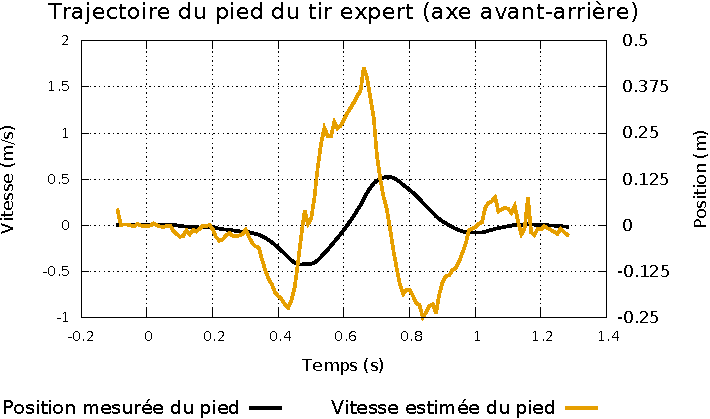
\includegraphics[type=pdf,ext=.pdf,read=.pdf,width=1.0\linewidth]{../plot/kickgreg_vel}
        \caption{\label{fig:kickgreg}
            Position et de vitesse du centre du pied de tir (en vol) 
            selon l'axe avant arrière $\bm{\vec{x}}$ 
            du meilleur mouvement de tir expert en 2016.
            Ce mouvement est manuellement mis au point sur le robot
            réel par essai-erreur afin de maximiser la portée du tir.
            On observe notamment la largeur du pic de vitesse ainsi
            que l'accélération positive du pied aux alentours du moment
            du contact supposé avec la balle.
        }
    \end{center}
\end{figure}

Les tout premiers tests de génération de tirs en simple support
stables se sont révélés entre $50\%$ et $75\%$ moins puissant que le tir expert. 
Ce tir utilisé lors de la compétition RoboCup est manuellement optimisé après de
longues séances d'expérimentation sur le robot réel.
Ce tir a donc fait l'objet d'une petite étude afin d'essayer de comprendre
les origines de sa puissance.
Les profils de position et de vitesse du pied de tir sont représentés sur
la figure \ref{fig:kickgreg}.
Après avoir enregistré et analysé l'intégralité des capteurs du robot lors
de ce mouvement, les observations suivantes peuvent être faites :
\begin{enumerate}
    \item Au moment de la collision entre le pied de tir et la balle,
        la vitesse effective mesurée du pied selon l'axe avant arrière est élevée
        (de l'ordre de $1.5~m.s^{-1}$).
        Dans tous ces travaux, il n'a jamais été possible d'obtenir 
        un mouvement stable par génération automatique avec une vitesse 
        aussi élevée.
        La théorie des chocs élastiques nous apprend en effet que
        l'énergie cinétique transmise à la balle est directement 
        fonction de cette vitesse.
    \item Cette vitesse reste élevée pendant une durée non négligeable
        ($200$ millisecondes). À l'inverse, les premières versions
        des mouvements générés, puisqu'ils tendent à minimiser 
        la consommation énergétique totale,
        présentaient un pic étroit de vitesse au moment du contact avec la balle.
        Intuitivement, en augmentant la durée de la zone à vitesse élevée, l'énergie
        transmise à la balle devient alors plus robuste aux variations de la position 
        réelle de la balle.
        En pratique au moment du tir, la balle n'est en effet jamais positionnée 
        parfaitement à l'emplacement désiré. 
    \item Toujours au moment du contact avec la balle, l'accélération
        du pied de tir est expérimentalement strictement positive vers l'avant.
        La trajectoire de vitesse du pied dans l'axe avant arrière forme donc un trapèze.
        Une petite simulation physique unidimensionnelle très simple a été réalisée 
        afin de mieux comprendre l'effet de la non rigidité de la balle 
        (simulation de la collision de deux solides mais séparés par un ressort).
        Lors du contact non idéal entre le pied et la balle, ces derniers se déforment
        et la durée du contact est coute mais non ponctuelle.
        Or durant cette courte période, l'accélération du pied est en mesure 
        de transmettre à la balle une certaine quantité de mouvement.
        En conclusion, on peut considérer que la vitesse de la balle après collision est dépendante : 
        de la vitesse d'impact élastique du pied, 
        de la rigidité des corps influençant la durée du 
        contact\footnote{
            Cette simple simulation met également en évidence qu'au delà d'une 
            certaine déformation, la vitesse finale de la balle diminue. 
            Il existerait bien une raideur optimale.
        } 
        et de l'accélération du pied au cours du contact transmettant 
        une énergie cinétique supplémentaire.
\end{enumerate}
Au regard de ces constats, les formes des mouvements de tir ont donc été modifiées.
Plus précisément, une trajectoire en trapèze sur la vitesse du pied de tir est imposée.
Toujours pour contrôler manuellement le compromis puissance-stabilité, les paramètres 
définissant la forme de ce trapèze (durée, vitesse initiale et finale de la zone de contact) 
sont laissés libres. Ils doivent ainsi être spécifiés avant toute génération de mouvement.

\subsection{Critères d'évaluation d'un mouvement et optimisation\label{sec:motion_fitness}}

Les mouvements sont synthétisés au travers d'un processus d'optimisation.
La qualité de chaque mouvement est alors définie par la somme pondérée d'un 
ensemble de critères, calculés grâce au modèle dynamique inverse du robot.
L'optimisation est ensuite effectuée par l'algorithme en boite noire CMA-ES 
(voir section \ref{sec:blackbox}).
L'intérêt de cet algorithme est de ne pas nécessiter le calcule du gradient de
toute la dynamique inverse (en gérant le cas du double support) 
ainsi que des différents critères.
Cette différentiation est toutefois possible et est largement pratiquée 
dans la littérature (par exemple par \cite{lengagne_planification_2009}). 
Moins efficace, notre approche nécessite des temps de calculs importants
(synthèse d'un mouvement entre une et quatre heures).

Le calcul du score (\textit{fitness}) d'un mouvement est effectué
de la manière suivante. Pour rappel, CMA-ES cherche à minimiser 
la valeur de ce score.
L'évaluation du mouvement est en pratique calculé sur un ensemble fini
de pas de temps, couvrant toute la longueur du mouvement.
Le score final est alors donné par la somme des scores intermédiaires.
Dans ces travaux, ce calcul est réalisé toutes les $0.01$ secondes.
Contrairement à la simulation (intégration numérique), la longueur de ce pas
de temps n'influence pas la précision des calculs. 
Cependant les contraintes sur le mouvement ne sont vérifiées que
sur ces pas de temps.
À chaque pas de temps, les étapes de calcul ci-dessous sont réalisées.

Tout d'abord, un ensemble de contraintes est imposé sur le mouvement.
Si ces contraintes ne sont pas respectées, le score du mouvement reçois
alors une forte pénalité (largement plus élevée que le score normal 
d'un mouvement respectant les contraintes).
À noter que cette pénalité n'est pas une constante. 
Pour aider l'algorithme à déterminer un gradient (direction vers laquelle se déplacer pour 
respecter la contrainte), cette pénalité est à chaque fois une fonction linéaire affine augmentant
avec la distance entre l'état actuel et la bordure de la contrainte.
Les contraintes suivantes sont imposées :
\begin{itemize}
    \item Tout d'abord, des contraintes dans l'espace cartésien sont imposées.
        La hauteur du buste et du pied en vol doivent toujours être au dessus du sol.
        L'orientation du buste et du pied en vol ne doivent pas dépasser $180$ degrés.
        Enfin, la position latérale du pied en vol ne doit pas se rapprocher trop
        de la jambe de support, afin d'éviter les auto collisions.
    \item Ensuite, les modèles géométrique et cinématique inverses sont calculés
        pour convertir dans l'espace articulaire les trajectoires définies 
        dans l'espace cartésien.
        Si la position cartésienne désirée n'est pas atteignable, 
        une forte pénalité est donnée.
        Pour estimer la distance à la bordure de la zone d'accessibilité, la
        \og distance \fg (sans signification physique) décrite à la section
        \ref{sec:modele_inverse} est utilisée\footnote{
            Quand les tirs désirés deviennent puissants, à cause du phénomène 
            de Runge des polynômes,
            il devient difficile de fournir manuellement à l'optimisation 
            un mouvement initial respectant les contraintes du modèle 
            géométrique inverse.
            L'introduction de ce critère a permis à l'optimisation de rapidement
            converger vers des mouvements réalisables. Chose très difficile
            à faire avec une exploration purement aléatoire de l'espace des paramètres.
        }.
        De plus, même si la configuration cartésienne désirée est atteignable,
        ce critère est utilisé pour imposer une marge de sécurité au respect de
        la contrainte du modèle géométrique inverse.
        En effet, comme les contraintes ne sont vérifiées que toutes les $0.01$~s,
        cette marge de sécurité (réglée manuellement) réduit les risques
        de dépasser la bordure d'accessibilité entre les pas de calcul.
    \item Enfin dans l'espace articulaire, un intervalle de position angulaire 
        est imposé sur chaque articulation.
        Ceci pour lutter contre des configurations indésirables et les auto collisions.
        Par exemple pour imposer le sens de pliage des genoux.
\end{itemize}
Ensuite selon l'état du mouvement, la dynamique inverse en simple ou double support  
(voir \ref{sec:dynamics_models} et \ref{sec:dynamics_constraints}) est calculée.
Grâce à l'information des couples présents au niveau de chaque articulation, 
les critères suivants sont déterminés :
\begin{itemize}
    \item En simple support, la distance sur le sol entre le ZMP et 
        le centre du pied de support est calculée (voir section \ref{sec:zmp}).
    \item En double support, la distance minimale sur le sol entre le ZMP et
        le segment reliant les centres des deux pieds de support est calculée.
    \item La modélisation des servomoteurs (section \ref{sec:model_servos})
        permet de calculer la tension électrique aux bornes de chaque moteur
        nécessaire pour créée les couples générés par le mouvement.
\end{itemize}
Le score du mouvement est alors un mélange pondéré de la distance moyenne
du ZMP et de la tension moyenne au niveau de chaque articulation.
L'idée est ici de minimiser la consommation énergétique en même tant
que de maximiser la stabilité du robot.
Ces valeurs moyennes permettent de donner une direction au gradient
pendant l'optimisation.

De plus, une condition sur la distance maximale du ZMP comparée à la taille
du pied de support permet d'imposer une contrainte de stabilité au mouvement.
De même, une condition sur la tension électrique maximale inférieure à la tension 
d'alimentation du robot impose que le mouvement pourra être \textit{théoriquement} 
suivit par les servomoteurs du robot.
Enfin même si le glissement est ici considéré comme inexistant, il sera
parfois intéressant en pratique de limiter au niveau du pied de support les forces
de contacts tangentielles ($\tau_\text{\textit{base\_x}}$ et $\tau_\text{\textit{base\_y}}$) 
ainsi que le couple en torsion ($\tau_\text{\textit{base\_yaw}}$).
Ceci pour éviter un glissement du pied de support au moment du tir.

\subsection{Simulateur dynamique\label{sec:motion_simulation}}

En raison des nombreuses imperfections, le comportement réel
mesuré sur le robot diffère significativement des trajectoires 
désirées, optimisées au travers du modèle dynamique inverse.
L'implémentation d'un simulateur dynamique a été commencé afin
de tenter de capturer et prédire l'effet de ces imperfections.

À terme, l'objectif final est le suivant : dans un premier temps, 
synthétiser la forme désirée d'un mouvement par optimisation de la dynamique 
inverse idéale du robot. L'intérêt est que cette étape
est bien plus rapide en temps de calcul que l'utilisation du simulateur dynamique.
Puis dans un second temps, raffiner et corriger toujours par optimisation le mouvement
au sein du simulateur, en \og trichant \fg sur les ordres envoyés aux moteurs de sorte 
à ce qu'ils prennent implicitement en compte par pré-compensation les défauts du robot.\\

La réimplémentation d'une simulation physique a été entreprise
avec le principal objectif de maitriser précisément chacune
des modélisations (dynamique, servomoteurs, contact) misent en oeuvre.
Inspiré par le formalisme de \cite{featherstone_rigid_2008} et \textit{RBDL},
ce simulateur se base sur la représentation du système par ses 
coordonnées généralisées (\textit{generalized coordinates}).
L'équation du mouvement est exprimée directement dans l'espace articulaire.
Les contraintes induites par les articulations sur les solides du robot
sont alors implicitement prises en compte.
Le simulateur \textit{DART} a par exemple fait ce choix d'implémentation.
D'autres simulateurs tels que \textit{ODE} et \textit{Bullet}
reposent sur l'utilisation des coordonnées maximales (\textit{maximal coordinates}).
La dynamique est alors résolue sous la forme d'un ensemble d'équations
différentielles sous contraintes explicites.\\

Ce simulateur est implémenté à l'aide des différents concepts présentés
à la section \ref{sec:model_dynamics}.
Afin de modéliser le fait que les deux pieds du robot peuvent selon
les cas ne pas être en contact avec le sol, la racine
de l'arbre mécanique est ici placée au niveau du buste du robot.
À chaque pas de simulation, les étapes suivantes sont effectuées :
\begin{itemize}
    \item Les hauteurs dans l'espace cartésien de tous les crampons
        sont calculées et comparées à l'altitude du sol pour détecter
        les possibles collisions.
    \item En prenant en compte l'ensemble des contraintes cinématiques actives ainsi
        que les couples moteurs créés sur chaque articulation, le modèle dynamique directe
        est calculé. Les accélérations au niveau de chaque degré de liberté sont déterminées.
    \item Les vitesses et positions de tous les degrés de liberté du système sont
        intégrées par une simple méthode d'Euler. L'utilisation de schémas d'intégration
        plus précis tels que \og Runge-Kutta 4 \fg rendent délicates la gestion 
        des modifications des contraintes cinématiques entres les pas de calcul.
    \item Les modèles des servomoteurs sont mis à jour. En fonction des ordres
        de positions angulaires, des frictions et potentiellement du modèle des 
        jeux mécaniques, les couples exercés en sortie de chaque servomoteur sont calculés.
\end{itemize}
Plus précisément au moment où une collision avec le sol d'un 
des crampons est détectée, les procédures suivantes sont exécutées :
\begin{itemize}
    \item Afin d'empêcher toute interpénétration dans le sol,
        des impulsions sont évaluées puis appliquées aux vitesses des 
        degrés de liberté du système.
    \item L'ensemble des contraintes actives sont recalculées
        par la résolution d'un problème LCP.
    \item Enfin l'ensemble des nouvelles contraintes cinématiques actives 
        est recalculé pour éviter toute redondance ou toute dégénérescence
        de la matrice des contraintes.\\
\end{itemize}

Le simulateur dynamique est en pratique configuré par de multiples
paramètres (paramètres inertiels, paramètres des servomoteurs).
Pour rapprocher les prédictions de la réalité, 
ces paramètres doivent être identifiés.
La littérature de ce domaine de recherche est très riche et n'a été que 
très peu étudiée dans ces travaux. 
Néanmoins il semblerait que de nombreuses méthodes 
(par exemple \cite{venture_dynamics_2008}, \cite{iwasaki_identification_2012} 
et \cite{traversaro_inertial_2013}) reposent sur l'utilisation
de plateformes ou capteurs de force $6$ axes internes ou externes au robot.
En l'absence de ces capteurs, une approche simple, similaire à celle 
proposée par \cite{urbann_rigid_2011} et se basant encore une fois 
sur CMA-ES a été mise en oeuvre.

Tout d'abord, plusieurs mouvements de tir différents 
(par exemple à plusieurs puissances ou positions de la balle) sont 
enregistrés sur le robot réel.
Les paramètres du simulateur sont alors optimisés avec CMA-ES de sorte à minimiser 
la distance quadratique moyenne entre la prédiction du simulateur et
le comportement observé pour chacune des articulations.
Il s'avère cependant que cette méthode présente de nombreux problèmes.
Les temps de calcul sont prohibitifs et dépassent typiquement les $24$~heures.
Ces temps étant directement proportionnel au nombre de mouvements d'apprentissage
enregistrés sur le robot et utilisés.
Malheureusement, le nombre de paramètres du simulateur à rechercher est élevé 
(entre $10$ et environ $300$ selon les modèles identifiés) ;
et il faudrait alors un grand nombre de mouvements d'apprentissage.
Or ceci est impossible au regard des temps de calculs.
En conséquence, l'identification est sujette au surapprentissage.
De plus amples expérimentations sont nécessaires pour tester la validité
de cette approche.

\subsection{Résultats préliminaires\label{sec:motion_results}}

Les premiers résultats de ces travaux 
peuvent être succinctement résumés par les points suivants :
\begin{itemize}
    \item Le processus d'optimisation a permis de trouver la posture statique
        en simple support minimisant la somme des couples des articulations du robot.
        Cette posture s'est en pratique révélée particulièrement stable 
        et a été utilisée comme pose initiale et finale des mouvements 
        de tir en simple support.
    \item L'optimisation de critères de stabilité fondés sur la dynamique inverse, 
        a permis la synthèse de mouvements de tir en simple support ainsi 
        que de mouvements de passage de double vers simple support.
        Le mouvement de tir en simple support stable le plus puissant
        a atteint une vitesse maximale théorique du pied de tir de $1.4~m.s^{-1}$
        (dans l'axe avant arrière).
        Le mouvement de passage d'une posture statique en double support 
        vers simple support s'est révélé robuste et répétable.
        Plus répétable que celui qui avait été manuellement mis au point 
        par l'équipe et utilisé de 2014 à 2015 par le tir en boucle fermée du robot.
    \item Même à faible puissance, les mouvements de tir 
        en double support synthétisés par optimisation de la 
        dynamique inverse ne sont pas stables sur le robot réel.
        Deux phénomènes sont principalement visibles.
        Dans un cas, au début du mouvement en passant sur un pied, 
        l'amplitude du basculement latéral du buste est trop importante 
        et le robot tombe alors sur le coté.
        Dans l'autre cas, le robot chute au moment où le pied
        de tir se pose sur le sol. 
        À cause des erreurs d'asservissement moteurs, 
        le pied n'est pas bien à plat par rapport au sol 
        et le robot est déstabilisé.
    \item Nous avons alors vérifié que notre choix de paramétrisation du mouvement 
        de tir en double support n'était pas la cause de ces problèmes de génération.
        Les paramètres du mouvement de tir en double support ont été identifiés afin
        de faire coïncider le plus possible les ordres moteurs générés par ce mouvement
        avec ceux engendrés par le tir expert, connu pour être stable.
        Une fois cette identification faite, il a été confirmé que le mouvement 
        était bien stable sur le robot physique.
        La paramétrisation choisi permet donc bien l'expression d'au moins un mouvement stable.
        Par contre, le critère de stabilité calculé à partir de la dynamique inverse (idéale)
        est mauvais sur ce mouvement. Il ne peut donc pas être sélectionné par l'optimisation.
    \item Après identification, le simulateur dynamique a été testé sur le
        problème de la correction du suivi de trajectoire.
        Sur un mouvement de tir en simple support peu puissant 
        (vitesse théorique maximale du pied de tir de $1.0~m.s^{-1}$ dans l'axe avant arrière),
        l'objectif est de réduire l'écart dans l'espace articulaire entre les trajectoires
        désirées (générées par optimisation de la dynamique inverse) et les trajectoires mesurées
        sur le robot physique.
        Pour ce faire, les ordres réellement envoyés aux moteurs sont modifiés.
        Sur le simulateur, les ordres envoyés aux moteurs sont optimisés de telle sorte que
        les trajectoires simulées se rapprochent des trajectoires désirées.
        Cette correction est comparée dans le tableau \ref{tab:motion_correction_feedforward}
        à la correction d'une commende en pré-compensation \textit{feedforward}\footnote{Le 
        \textit{feedforward} utilise le contrôle proportionnel du servomoteur 
        pour imposer un couple en sortie désiré, calculé par dynamique inverse 
        pour suivre le mouvement.}.
        La correction optimisée dans le simulateur améliore le suivi de trajectoire
        en simulation et sur le robot réel, mieux que le \textit{feedforward}.
        À noter que le \textit{feedforward} se base également sur les mêmes 
        paramètres inertiels que le simulateur.
\end{itemize}

\begin{table}[htb!]
    \centerfloat
    \small
    \begin{tabular}{|l|l|l|}
        \hline
        Mouvement & Erreur moyenne (degrés) & Erreur maximale (degrés) \\
        \hline
        \multicolumn{3}{|c|}{Dans le simulateur (identifié)} \\
        \hline
        Original & 2.56 & 17.9 \\
        Feedforward & 1.20 & 9.61 \\
        Simulateur & 0.45 & 3.21 \\
        \hline
        \multicolumn{3}{|c|}{Sur le robot Sigmaban} \\
        \hline
        Original & 2.46 & 22.1 \\
        Feedforward & 0.88 & 12.0 \\
        Simulateur & 0.71 & 5.94 \\
        \hline
    \end{tabular}
    \caption{\label{tab:motion_correction_feedforward}
        Comparaison au niveau des articulations de l'erreur de suivi
        de trajectoire d'un mouvement désiré.
        Le mouvement est un tir peu puissant en simple support 
        (vitesse maximale du pied de tir de $1.0~m.s^{-1}$ dans l'axe avant arrière).
        Le mouvement original sans correction, le mouvement corrigé par \textit{feedforward}
        et le mouvement corrigé par optimisation dans le simulateur sont comparés.
        En haut, en simulation et en bas, sur le robot Sigmaban réel.
        L'erreur moyenne considère toutes les articulations le long
        de toute la trajectoire.
        L'erreur maximale correspond à l'écart le plus grand le long de la trajectoire
        et parmi toutes les articulations.
    }
\end{table}

